\chapter{Visualization with Seaborn\label{Ch36}}
\section{Exploring Seaborn Plots}
The main idea of Seaborn is that it provides high-level commands to create a variety
of plot types useful for statistical data exploration, and even some statistical model
fitting.

Let’s take a look at a few of the datasets and plot types available in Seaborn. Note that
all of the following could be done using raw Matplotlib commands (this is, in fact,
what Seaborn does under the hood), but the Seaborn API is much more convenient.

\subsection*{Histograms, KDE, and Densities}
Often in statistical data visualization, all you want is to plot histograms and joint distributions of variables. We have seen that this is relatively straightforward in Matplotlib.


Rather than just providing a histogram as a visual output, we can get a smooth estimate of the distribution using kernel density estimation,
which Seaborn does with \verb|sns.kdeplot|.

If we pass $x$ and $y$ columns to kdeplot, we instead get a two-dimensional visualization of the joint density.

We can see the joint distribution and the marginal distributions together using
\verb|sns.jointplot|.

\subsubsection*{Pair Plots}
When you generalize joint plots to datasets of larger dimensions, you end up with
\textbf{pair plots}(矩阵图). These are very useful for exploring correlations between multidimensional
data, when you’d like to plot all pairs of values against each other.

Visualizing the multidimensional relationships among the samples is as easy as calling \verb|sns.pairplot|.

\subsection*{Faceted Histograms}
Sometimes the best way to view data is via histograms of subsets. Seaborn’s \verb|FacetGrid| makes this simple.

\section{Categorical Plots}
Categorical plots can be useful for this kind of visualization as well. These allow you
to view the distribution of a parameter within bins defined by any other parameter.

\subsection*{Joint Distributions}
Similar to the pair plot we saw earlier, we can use sns.jointplot to show the joint
distribution between different datasets, along with the associated marginal distributions.(see \autoref{A joint distribution plot})

The joint plot can even do some automatic kernel density estimation and regression, as shown in \autoref{A joint distribution plot with a regression fit}.

\begin{figure}
    \centering
    \begin{subfigure}[b]{.45\textwidth}
        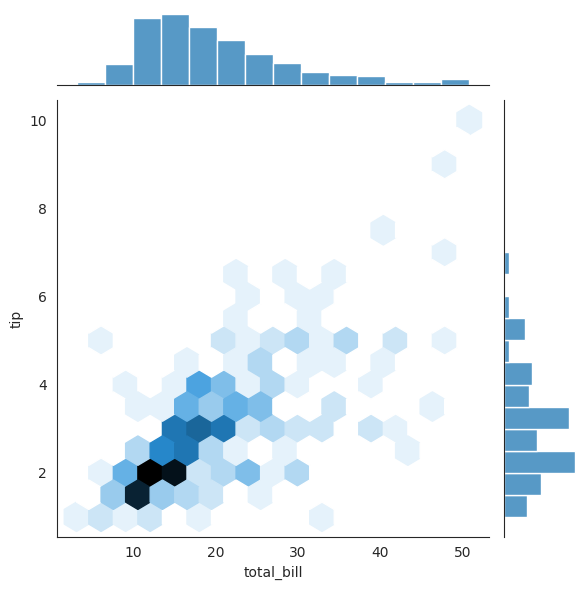
\includegraphics[width=\textwidth]{../Figures/A joint distribution plot.png}
        \caption{A joint distribution plot}
        \label{A joint distribution plot}
    \end{subfigure}
    \hfill
    \begin{subfigure}[b]{.45\textwidth}
        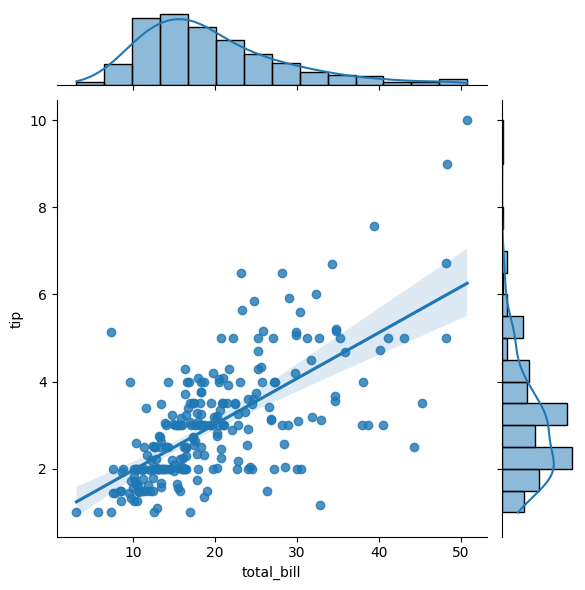
\includegraphics[width=\textwidth]{../Figures/A joint distribution plot with a regression fit.png}
        \caption{A joint distribution plot with a regression fit}
        \label{A joint distribution plot with a regression fit}
    \end{subfigure}
    \caption{Joint Distributions}
\end{figure}

\subsection*{Bar Plots}
Time series can be plotted using \verb|sns.catplot|. We can learn more by looking at the factor of data of each of these categories.

For more information on plotting with Seaborn, see the \href{http://seaborn.pydata.org/}{Seaborn documentation}, and
particularly the \href{https://seaborn.pydata.org/examples/index.html}{example gallery}.

\section{用Basemap可视化地理数据}
地理数据可视化是数据科学中一种十分常见的可视化类型。Matplotlib 做此类可视化的主
要工具是 Basemap 工具箱。

\subsection{地图投影}
当你想使用地图时,首先要做的就是确定地图的投影类型。你可能已经知道,像地球这样
的球体,可以通过球面透视法将三维球面投影成一个二维平面,不会造成变形,也不会破坏其连续性。

\subsubsection*{圆柱投影}
圆柱投影(cylindrical projection)是最简单的地图投影类型,纬度线与经度线分别映射
成水平线与竖直线。采用这种投影类型的话,赤道区域的显示效果非常好,但是南北极
附近的区域就会严重变形。由于纬度线的间距会因圆柱投影的不同而不同,所以就有了
不同的投影属性和南北极附近不同的变形程度。等距圆柱投
影(cyl),不同纬度在子午线方向的间距保持不变。另外两种圆柱投影是墨卡托(Mercator,
projection='merc')投影和圆柱等积(cylindrical equal-area,projection='cea')投影。
\subsubsection*{伪圆柱投影}
伪圆柱投影(pseudo-cylindrical projection)的经线不再必须是竖直的,这样可以使南北
极附近的区域更加真实。摩尔威德(Mollweide,projection='moll')投影就是这类投影
的典型代表,它所有的经线都是椭圆弧线,如图 4-105 所示。这么做是为了保留地图原
貌——虽然南北极附近的区域还有一些变形,但是通过一些区域小图可以反映真实情况。
其他伪圆柱投影类型有正弦(sinusoidal,projection='sinu')投影和罗宾森(Robinson,
projection='robin')投影。
\subsubsection*{透视投影}
透视投影(perspective projection)是从某一个透视点对地球进行透视获得的投影,就好像
你站在太空中某一点给地球照相一样(通过技术处理,有些投影类型的透视点可以放在地
球上)。一个典型示例是正射(orthographic,projection='ortho')投影,从无限远处观
察地球的一侧。因此,这种投影一次只能显示半个地球。其他的透视投影类型还有球心(gnomonic,projection='gnom') 投 影 和 球 极 平 面(stereographic,projection='stere')
投影。这些投影经常用于显示地图的较小面积区域。

\subsubsection*{圆锥投影}
圆锥投影(conic projection)是先将地图投影成一个圆锥体,然后再将其展开。这样做虽
然可以获得非常好的局部效果,但是远离圆锥顶点的区域可能会严重变形。一个典型示例
就是兰勃特等角圆锥投影(Lambert conformal conic projection,projection='lcc'),也就
是我们之前见到的北美洲地图。这种方法将地图投影成一个由两条标准纬线(用 Basemap
里的 lat\_1 与 lat\_2 参数设置)构成的圆锥,这两条纬线距离是经过精心挑选的,在两条
标准纬线之内比例尺逐渐减小,在两线之外的比例尺逐渐增大。其他常用的圆锥投影还有
等距圆锥(equidistant conic,projection='eqdc')投影和阿尔伯斯等积圆锥(Albers equalarea,projection='aea')投影。圆锥投影和透视投影一样,适合显示较
小与中等区域的地图。